% =====================================================================
%  Manual: preparación, captura y despliegue de la imagen maestra CPE
%  Compilar desde esta carpeta:  latexmk -pdf -g Manual_Imagen_Maestra_V4.tex
%  Las fotografías se leen de ../Imagenes manual/
% =====================================================================
\documentclass[11pt,a4paper]{report}

\usepackage[utf8]{inputenc}
\usepackage[T1]{fontenc}
\usepackage[spanish,es-tabla]{babel}
\usepackage{lmodern}
\usepackage{microtype}
\usepackage[margin=2.3cm,headheight=26pt]{geometry}
\usepackage{graphicx}
\usepackage{float}
\usepackage{caption}
\usepackage{subcaption}
\usepackage{booktabs}
\usepackage{tabularx}
\usepackage{enumitem}
\usepackage[table]{xcolor}
\usepackage{fancyhdr}
\usepackage{titlesec}
\usepackage[most]{tcolorbox}
\usepackage[hidelinks]{hyperref}

\graphicspath{{../Imagenes manual/}{logos/}}

% ---------------------------------------------------------------------
%  Colores y estilo
% ---------------------------------------------------------------------
\definecolor{azulcpe}{HTML}{0B5CAD}
\definecolor{grisclaro}{HTML}{F2F4F7}
\definecolor{rojoaviso}{HTML}{B42318}
\definecolor{verdeok}{HTML}{067647}
\definecolor{amarillo}{HTML}{B54708}

\titleformat{\chapter}[display]
  {\normalfont\bfseries\color{azulcpe}\raggedright}
  {\large\MakeUppercase{\chaptertitlename}\ \thechapter}
  {4pt}{\Huge}
\titleformat{\section}{\normalfont\Large\bfseries\color{azulcpe}}{\thesection}{0.8em}{}
\titleformat{\subsection}{\normalfont\large\bfseries}{\thesubsection}{0.8em}{}

\captionsetup{font=small,labelfont={bf,color=azulcpe},margin=1cm}
\captionsetup[sub]{font=footnotesize}

\pagestyle{fancy}
\fancyhf{}
\fancyhead[L]{\raisebox{-0.3\height}{
\includegraphics[height=0.75cm]{unal_escudo_verde.png}}%
  \hspace{6pt}\small\color{gray}Manual de imagen maestra CPE}
\fancyhead[R]{\small\color{gray}\leftmark}
\fancyfoot[C]{\small\thepage}
\renewcommand{\headrulewidth}{0.4pt}

\setlist[enumerate]{leftmargin=*,itemsep=3pt}
\setlist[itemize]{leftmargin=*,itemsep=2pt}

% ---------------------------------------------------------------------
%  Comandos propios
% ---------------------------------------------------------------------
% Barra invertida para rutas de Windows (permite cortar la línea después)
\newcommand{\bs}{\textbackslash\allowbreak{}}
% Botón o elemento de la interfaz
\newcommand{\boton}[1]{\textsf{\textbf{#1}}}
% Tecla
\newcommand{\tecla}[1]{\tcbox[on line,boxsep=1pt,left=3pt,right=3pt,top=0pt,bottom=0pt,
  colback=grisclaro,colframe=gray!60,boxrule=0.4pt,arc=2pt]{\texttt{\small #1}}}

% Fotografía a ancho completo: \foto[ancho]{archivo}{pie}{etiqueta}
\newcommand{\foto}[4][0.88\textwidth]{%
  \begin{figure}[H]
    \centering
    \includegraphics[width=#1,height=0.42\textheight,keepaspectratio]{#2}
    \caption{#3}\label{#4}
  \end{figure}}

% Dos fotografías lado a lado
\newcommand{\dosfotos}[6]{%
  \begin{figure}[H]
    \centering
    \begin{subfigure}[t]{0.49\textwidth}
      \centering\includegraphics[width=\linewidth]{#1}\caption{#2}
    \end{subfigure}\hfill
    \begin{subfigure}[t]{0.49\textwidth}
      \centering\includegraphics[width=\linewidth]{#3}\caption{#4}
    \end{subfigure}
    \caption{#5}\label{#6}
  \end{figure}}

% Cajas de aviso
\newtcolorbox{importante}[1][Importante]{enhanced,breakable,
  colback=rojoaviso!5,colframe=rojoaviso,fonttitle=\bfseries,title=#1,
  boxrule=0.6pt,arc=2pt,left=6pt,right=6pt}
\newtcolorbox{nota}[1][Nota]{enhanced,breakable,
  colback=azulcpe!5,colframe=azulcpe,fonttitle=\bfseries,title=#1,
  boxrule=0.6pt,arc=2pt,left=6pt,right=6pt}
\newtcolorbox{resultado}[1][Resultado esperado]{enhanced,breakable,
  colback=verdeok!5,colframe=verdeok,fonttitle=\bfseries,title=#1,
  boxrule=0.6pt,arc=2pt,left=6pt,right=6pt}

% =====================================================================
\begin{document}

% ---------------------------------------------------------------------
%  Portada
% ---------------------------------------------------------------------
\begin{titlepage}
  \centering
  
\includegraphics[width=3.6cm]{unal_logosimbolo_verde.png}\\[1cm]
  {\color{azulcpe}\rule{\linewidth}{1.2pt}}\\[0.8cm]
  {\Huge\bfseries\color{azulcpe} Manual de imagen maestra de Windows\par}
  \vspace{0.4cm}
  {\LARGE Preparación, captura y despliegue\par}
  \vspace{0.5cm}
  {\color{azulcpe}\rule{\linewidth}{1.2pt}}\\[1.2cm]
  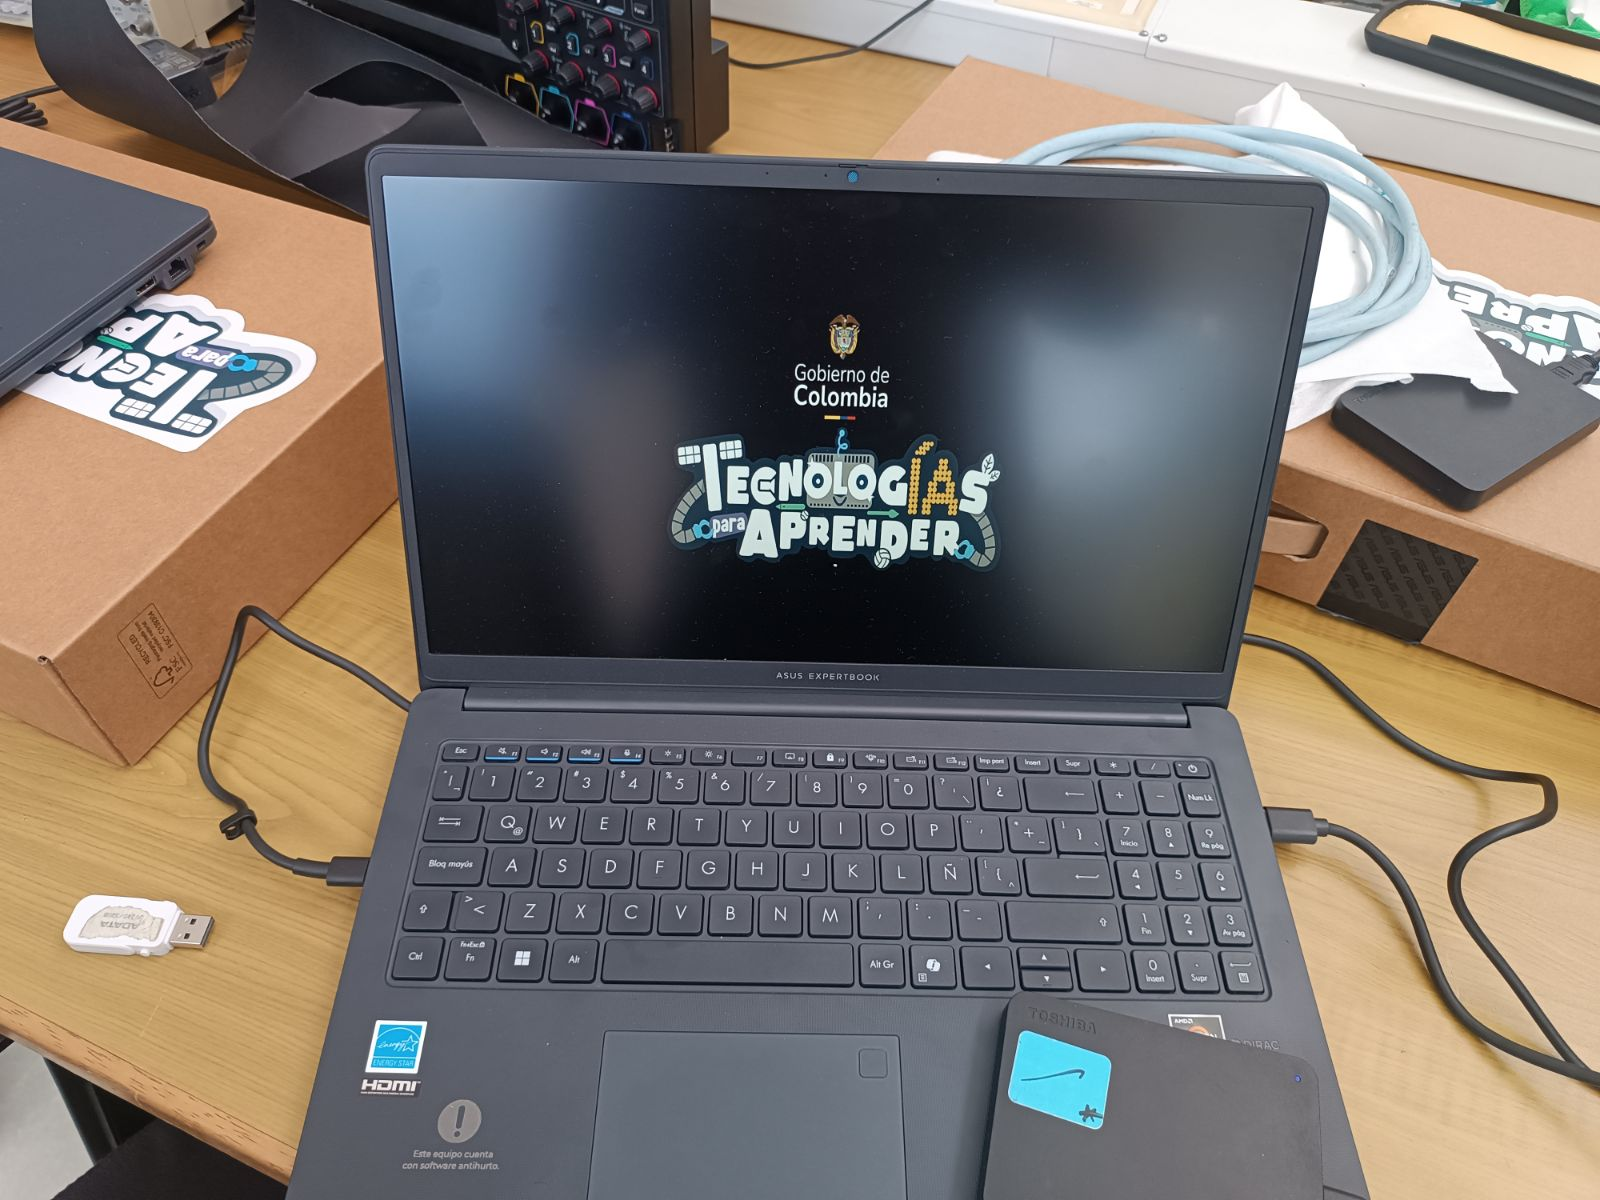
\includegraphics[width=0.62\textwidth]{Image_20261020_1306382292668009792503941.jpeg}\\[0.8cm]
  {\large Herramienta \texttt{ImagenMaestra.cmd} con Hiren's BootCD PE\par}
  \vspace{0.3cm}
  {\large Equipo de referencia: ASUS ExpertBook\par}
  \vfill
  {\large Repositorio \texttt{Imagenes\_Maestras\_CPE}\par}
  \vspace{0.2cm}
  {\large Noviembre de 2026\par}
\end{titlepage}

\tableofcontents
\clearpage

% =====================================================================
\chapter{Introducción}
% =====================================================================

Este manual explica, paso a paso y con fotografías del proceso real, cómo se
crea una \textbf{imagen maestra de Windows} en un equipo de referencia
ASUS ExpertBook y cómo se despliega después en los equipos de destino. Todo el
proceso se hace con un único script, \texttt{ImagenMaestra.cmd}, que abre una
interfaz con una pestaña para cada fase.

\begin{table}[H]
  \centering
  \small
  \rowcolors{2}{grisclaro}{white}
  \begin{tabularx}{\textwidth}{@{}l l l >{\raggedright\arraybackslash}X@{}}
    \toprule
    \textbf{Fase} & \textbf{Pestaña o programa} & \textbf{Dónde se ejecuta} & \textbf{Resultado} \\
    \midrule
    1. Preparación & 1. Preparar y Sysprep & Windows, equipo de referencia &
      Equipo limpio, en es-MX, con una sola cuenta y apagado por Sysprep \\
    2. Captura & 2. Capturar imagen & Hiren's, equipo de referencia &
      Archivo \texttt{Imagenes\bs <nombre>.wim} con Windows y las particiones extra \\
    3. Despliegue & 3. Desplegar imagen & Hiren's, cada equipo de destino &
      Disco particionado, Windows aplicado y nombre del equipo = serial \\
    4. Verificación & \texttt{CuentasCPE.cmd} & Windows, cada equipo de destino &
      Informe en \texttt{ScriptsEducativos\bs Logs\bs} \\
    \bottomrule
  \end{tabularx}
  \caption{Fases del proceso.}
\end{table}

\section{Qué hace la herramienta}

\begin{itemize}
  \item Deja el equipo de referencia con \textbf{es-MX como único idioma},
        una sola cuenta (\textbf{AdministradorCPE}) y un \textbf{fondo común}
        para todas las cuentas.
  \item Cuando la preparación necesita reiniciar, lo indica, pregunta
        \emph{¿Reiniciar ahora?} y \textbf{continúa sola} al volver a iniciar
        sesión (sección~\ref{sec:idioma}).
  \item Captura en un solo archivo \texttt{.wim} la partición de Windows y las
        particiones de recuperación y datos.
  \item Despliega la imagen en otros equipos, aunque tengan un disco más
        pequeño, y les pone como nombre el \textbf{serial de la BIOS}
        (sección~\ref{sec:nombre}).
\end{itemize}

\section{Materiales utilizados}

\begin{table}[H]
  \centering
  \small
  \rowcolors{2}{grisclaro}{white}
  \begin{tabularx}{\textwidth}{@{}l X@{}}
    \toprule
    \textbf{Elemento} & \textbf{Detalle} \\
    \midrule
    Equipo de referencia & ASUS ExpertBook, AMD Ryzen 5 7535HS, 16 GB de RAM,
      SSD NVMe Samsung de 1 TB, firmware UEFI \\
    USB de arranque & Memoria con Hiren's BootCD PE (Windows 11 PE x64),
      etiqueta \texttt{HBCD\_PE\_x64} \\
    Disco externo & Toshiba de 1 TB (931 GB útiles), NTFS, USB 3.0 \\
    Herramienta & Carpeta \texttt{Img\_V4} (copia del repositorio) en la raíz del disco externo \\
    Licencias & Una licencia de Windows por cada equipo de destino \\
    \bottomrule
  \end{tabularx}
  \caption{Hardware y software empleados.}
\end{table}

\foto[0.8\textwidth]{1000214233.jpeg}
  {Montaje de trabajo: equipo de referencia con la memoria USB de Hiren's
   (izquierda) y el disco externo Toshiba (derecha) conectados.}
  {fig:montaje}

\begin{importante}
El despliegue \textbf{borra por completo} el disco de destino. Antes de
confirmar, revise siempre el número, modelo y tamaño del disco seleccionado.
\end{importante}

% =====================================================================
\chapter{Obtención de la herramienta}
% =====================================================================

\section{Descargar el repositorio}

\begin{enumerate}
  \item Abra el repositorio \texttt{Imagenes\_Maestras\_CPE} en GitHub:\\[2pt]
        {\color{azulcpe}\underline{\url{https://github.com/DarkSpartan345/Imagenes_Maestras_CPE}}}\\[2pt]
        y pulse el botón verde \boton{Code} (figura~\ref{fig:github}).
  \item En el menú que aparece, copie la dirección HTTPS para clonarlo con Git,
        o elija \boton{Download ZIP} para descargarlo como archivo comprimido
        (figura~\ref{fig:clonar}).
\end{enumerate}

\foto{image(1).png}
  {Página del repositorio en GitHub. El botón \textsf{Code} está marcado en rojo.}
  {fig:github}

\foto{image(2).png}
  {Menú \textsf{Code}: copiar la URL HTTPS o descargar el ZIP.}
  {fig:clonar}

\section{Copiar la carpeta al disco externo}\label{sec:copiar}

Copie la carpeta completa a la \textbf{raíz de un disco externo NTFS}. En este
caso se llamó \texttt{Img\_V4}. El nombre no importa: la herramienta
detecta sola su carpeta.

\foto[0.7\textwidth]{image(3).png}
  {Contenido de la carpeta en el disco externo. \texttt{ImagenMaestra.cmd} es
   el script que se usa en todas las fases.}
  {fig:carpeta}

\begin{table}[H]
  \centering
  \small
  \rowcolors{2}{grisclaro}{white}
  \begin{tabularx}{\textwidth}{@{}l X@{}}
    \toprule
    \textbf{Carpeta o archivo} & \textbf{Para qué sirve} \\
    \midrule
    \texttt{ImagenMaestra.cmd} & Preparar, capturar y desplegar \\
    \texttt{CuentasCPE.cmd} & Verificar cada equipo ya desplegado (en Windows) \\
    \texttt{ScriptsEducativos\bs} & \texttt{Verificar-Equipo.ps1}, que lanza \texttt{CuentasCPE.cmd}; informes en \texttt{Logs\bs} \\
    \texttt{Imagenes\bs} & Imágenes \texttt{.wim} capturadas (y \texttt{.swm} si se dividen) \\
    \texttt{Drivers\bs} & (Opcional) drivers \texttt{.inf} que se inyectan al desplegar \\
    \texttt{Respuesta\bs} & (Opcional) un \texttt{unattend.xml} propio \\
    \texttt{Logs\bs} & Registros de DISM y de cada fase (se crea solo) \\
    \texttt{Scratch\bs} & Carpeta temporal de DISM (se crea y se borra sola) \\
    \texttt{LEEME.txt}, \texttt{README*.md} & Manual de uso, protocolo de pruebas y descripción técnica \\
    \bottomrule
  \end{tabularx}
  \caption{Estructura de la carpeta de trabajo.}
\end{table}

\begin{nota}[Si la ventana no abre]
Si la interfaz gráfica no se puede abrir (por ejemplo, en un WinPE sin .NET),
el script muestra un \textbf{menú de texto} con las mismas acciones
(opciones 1 a 8). Las preguntas se responden con \texttt{S} o \texttt{N}.
\end{nota}

% =====================================================================
\chapter{Fase 1: preparación del equipo de referencia}
\chaptermark{Fase 1: preparación}
% =====================================================================

Esta fase se ejecuta en el \textbf{Windows del equipo de referencia}, después
de instalar y personalizar todos los programas y contenidos que llevará la
imagen.

\section{Antes de empezar}

\begin{itemize}
  \item Deje el equipo personalizado: programas, contenidos educativos, fondo
        de pantalla y accesos directos. El fondo de la cuenta con la que
        trabaja será el fondo común de todas las cuentas.
  \item \textbf{Desconecte internet}, para que la Microsoft Store no actualice
        aplicaciones y bloquee Sysprep. La única excepción es cuando falta el
        idioma es-MX: esa vez sí se necesita internet para descargarlo.
  \item \textbf{Quite el cifrado del dispositivo} (BitLocker), como se indica
        a continuación. Con la unidad \texttt{C:} cifrada la imagen no se puede
        capturar.
  \item Conecte el disco externo y déjelo conectado durante toda la fase,
        incluidos los reinicios.
\end{itemize}

\subsection*{Quitar el cifrado del dispositivo}\label{sec:descifrar}

\begin{enumerate}
  \item Busque \emph{configuración} en el menú Inicio y abra la aplicación
        \boton{Configuración}. En el menú de la izquierda elija
        \boton{Privacidad y seguridad} (figura~\ref{fig:cifrado-abrir}).
\end{enumerate}

\dosfotos{image(20).png}{Buscar y abrir \textsf{Configuración}.}
  {image(21).png}{Entrar en \textsf{Privacidad y seguridad}.}
  {Acceso a la configuración de privacidad y seguridad.}
  {fig:cifrado-abrir}

\begin{enumerate}[resume]
  \item En la sección \emph{Seguridad} pulse \boton{Cifrado de dispositivo}.
        Si aparece en \emph{Activado}, pulse el interruptor para desactivarlo
        (figura~\ref{fig:cifrado-desactivar}).
\end{enumerate}

\dosfotos{image(22).png}{Opción \textsf{Cifrado de dispositivo}.}
  {image(23).png}{Cifrado activado: pulse el interruptor.}
  {Desactivación del cifrado del dispositivo.}
  {fig:cifrado-desactivar}

\begin{enumerate}[resume]
  \item Confirme con \boton{Desactivar} (figura~\ref{fig:cifrado-confirmar}).
\end{enumerate}

\foto[0.55\textwidth]{image(24).png}
  {Confirmación para desactivar el cifrado.}
  {fig:cifrado-confirmar}

\begin{enumerate}[resume]
  \item Espere a que termine el descifrado; puede tardar varios minutos. Al
        final la opción queda en \emph{Desactivado}
        (figura~\ref{fig:cifrado-listo}).
\end{enumerate}

\foto[0.8\textwidth]{image(25).png}
  {Cifrado del dispositivo desactivado.}
  {fig:cifrado-listo}

\section{Elegir las opciones}\label{sec:opciones}

\begin{enumerate}
  \item En el disco externo, haga doble clic en \texttt{ImagenMaestra.cmd} y
        concédale los permisos de administrador que solicita al abrirse.
  \item Vaya a la pestaña \boton{1. Preparar y Sysprep}.
  \item Marque las opciones señaladas en rojo en la figura~\ref{fig:prep-opciones}.
\end{enumerate}

\foto[0.8\textwidth]{image(4).png}
  {Pestaña \textsf{Preparar y Sysprep} con las opciones usadas
   (marcadas en rojo).}
  {fig:prep-opciones}

\begin{table}[H]
  \centering
  \small
  \rowcolors{2}{grisclaro}{white}
  \begin{tabularx}{\textwidth}{@{}>{\raggedright\arraybackslash}p{6.2cm} c X@{}}
    \toprule
    \textbf{Opción} & \textbf{Usada} & \textbf{Qué hace} \\
    \midrule
    Quitar automáticamente las apps de la Store que bloquean Sysprep & Sí &
      Quita las aplicaciones instaladas solo para un usuario, que hacen fallar Sysprep \\
    Limpieza profunda de componentes & No &
      DISM \texttt{/ResetBase}: reduce el tamaño de la imagen, pero es lenta \\
    Fondo de esta cuenta en todas las cuentas (obligatorio) & Sí &
      Copia el fondo a \texttt{C:\bs Windows\bs Web\bs Wallpaper\bs CPE\bs} y lo bloquea
      para todas las cuentas, también las nuevas \\
    Dejar SOLO la cuenta AdministradorCPE + \emph{Sin contraseña} & Sí &
      Renombra o crea AdministradorCPE y borra las demás cuentas con su perfil \\
    Equipos desplegados sin configuración inicial & Sí &
      Los equipos arrancan directo al inicio de sesión \\
    \bottomrule
  \end{tabularx}
  \caption{Opciones de la pestaña 1.}
\end{table}

\begin{nota}[Contraseña de AdministradorCPE]
Si quiere una contraseña, desmarque \emph{Sin contraseña} y escríbala dos veces
(\emph{Contraseña} y \emph{Repetir}). Se guarda cifrada. Si AdministradorCPE ya
existe, dejar el campo vacío significa \textbf{no cambiar} su contraseña.
\end{nota}

\begin{enumerate}[resume]
  \item Pulse \boton{Preparar y ejecutar Sysprep}.
  \item Lea el resumen de confirmación. Indica cómo quedará la cuenta
        AdministradorCPE, qué cuentas se eliminarán con sus perfiles
        (aquí \emph{Estudiante} y \emph{Estudiantes}) y que el equipo se
        apagará al terminar. Pulse \boton{Sí} (figura~\ref{fig:prep-confirmar}).
\end{enumerate}

\foto[0.6\textwidth]{image(13).png}
  {Confirmación antes de ejecutar la preparación.}
  {fig:prep-confirmar}

\section{Comprobaciones automáticas}

El script revisa el equipo antes de tocar nada. En la consola inferior se ve
cada comprobación con \texttt{[OK]}, \texttt{[!]} (aviso), \texttt{[X]} (error)
o \textcolor{amarillo}{\texttt{[REINICIO]}}:

\begin{enumerate}
  \item Que el equipo no esté unido a un dominio.
  \item Que la unidad \texttt{C:} no esté cifrada con BitLocker.
  \item Que no haya reinicios pendientes de Windows Update.
  \item Que el almacenamiento reservado esté desactivado.
  \item Que el idioma de la imagen sea español latinoamericano (es-MX).
\end{enumerate}

\foto{Idioma.png}
  {Comprobaciones automáticas. Las cuatro primeras salen en verde; el idioma
   es-MX no está instalado y empieza a descargarse.}
  {fig:prep-comprobaciones}

\section{Idioma es-MX y reinicios guiados}\label{sec:idioma}

La imagen siempre queda con \textbf{es-MX como único idioma de pantalla}. Si el
equipo no lo tiene, el script lo descarga (necesita internet), lo fija como
idioma de pantalla, formato regional y teclado, y pide reiniciar para que
Windows lo aplique.

Pedir un reinicio \textbf{no es un error}. El script
muestra el motivo en amarillo con \texttt{[REINICIO]} y abre la ventana
\emph{Hace falta reiniciar el equipo para continuar (no es un error)}
(figura~\ref{fig:prep-reinicio}).

\foto{idioma_2.png}
  {Aviso de reinicio tras instalar es-MX. Pulse \textsf{Yes} para reiniciar
   en 5 segundos.}
  {fig:prep-reinicio}

\subsection*{Qué hacer cuando pide reiniciar}

\begin{enumerate}
  \item Pulse \boton{Yes} en \emph{¿Reiniciar ahora?}. El equipo reinicia en
        5 segundos. Si pulsa \boton{No}, reinicie usted más tarde: la
        continuación queda registrada igual.
  \item Inicie sesión con la \textbf{misma cuenta} (en la figura,
        \emph{Estudiantes}). Deje conectado el disco externo.
  \item La ventana de \texttt{ImagenMaestra.cmd} se abre sola en la pestaña 1 y
        pregunta: \emph{Preparar se detuvo para reiniciar el equipo:
        <motivo>. ¿Continuar ahora Preparar con las mismas opciones?}
  \item \textbf{Desconecte internet} (salvo que aún falte descargar el idioma)
        y pulse \boton{Sí}. No vuelve a pedir la contraseña.
\end{enumerate}

\begin{table}[H]
  \centering
  \small
  \rowcolors{2}{grisclaro}{white}
  \begin{tabularx}{\textwidth}{@{}l X@{}}
    \toprule
    \textbf{Motivo del reinicio} & \textbf{Qué pasó} \\
    \midrule
    Reinicio pendiente de Windows Update & Hay actualizaciones a medio instalar \\
    Almacenamiento reservado & Se desactivó y estaba en uso (evita el error 0x800F0975) \\
    Idioma recién instalado & es-MX se descargó y se fijó; Windows lo aplica al reiniciar \\
    Idiomas desinstalados & En la segunda pasada se quitaron los demás idiomas (por ejemplo, en-US) \\
    \bottomrule
  \end{tabularx}
  \caption{Casos en que la preparación pide reiniciar (código de salida 4).}
\end{table}

En la siguiente pasada la comprobación de idioma sale correcta:
\texttt{La imagen queda en es-MX como único idioma de pantalla}. El español de
España (es-ES) puede quedar instalado \emph{solo como reserva} de es-MX; es
normal. Después el script quita las aplicaciones de la Store que bloquean
Sysprep (figura~\ref{fig:prep-idioma-ok}).

\foto{Idioma_3.png}
  {Idioma correcto: en-US desinstalado y es-MX como único idioma de
   pantalla. El proceso continúa con las apps de la Store.}
  {fig:prep-idioma-ok}

\begin{nota}[Freno contra bucles y cancelación]
\begin{itemize}
  \item Si la preparación pide reiniciar \textbf{3 veces seguidas por el mismo
        motivo}, se detiene y desactiva la continuación automática. Revise el
        motivo indicado antes de volver a intentarlo.
  \item Si responde \boton{No} a \emph{¿Continuar ahora Preparar?}, la
        continuación se borra y la ventana ya no se abre sola. Puede volver a
        pulsar \boton{Preparar y ejecutar Sysprep} cuando quiera.
  \item Si no hay internet y es-MX no se puede instalar, la ventana pregunta
        si aceptar el idioma actual.
\end{itemize}
\end{nota}

\section{Limpieza y Sysprep}\label{sec:sysprep}

Con todo en orden, el script:

\begin{enumerate}
  \item Deja solo la cuenta AdministradorCPE. Las cuentas que están en uso y
        no se pueden borrar se anotan para borrarlas en el primer arranque de
        cada equipo desplegado.
  \item Aplica el \textbf{fondo común} a todas las cuentas.
  \item Limpia los temporales, la papelera y las \textbf{cachés de la GPU}
        (AMD, NVIDIA, Intel), que pueden causar el error 1299 de DISM.
  \item Crea el archivo \texttt{C:\bs Windows\bs System32\bs Sysprep\bs unattend.xml},
        que omite la configuración inicial con idioma es-MX, teclado
        latinoamericano y zona horaria de México.
  \item Borra la continuación automática (\texttt{RunOnce} y el archivo de
        opciones) para que \textbf{no quede dentro de la imagen}.
  \item Ejecuta:\\[2pt]
        \texttt{\small sysprep.exe /generalize /oobe /shutdown /quiet}\\
        \texttt{\small\hspace*{2em}/unattend:C:\bs Windows\bs System32\bs Sysprep\bs unattend.xml}
\end{enumerate}

\foto[0.5\textwidth]{image(19).png}
  {Sysprep en ejecución (fase de limpieza de complementos).}
  {fig:sysprep}

\begin{importante}[Al terminar Sysprep]
El equipo se \textbf{apaga solo}. \textbf{No lo encienda en Windows}: si
arranca Windows, Sysprep se consume y hay que preparar de nuevo. El siguiente
arranque debe ser desde la memoria USB de Hiren's.
\end{importante}

% =====================================================================
\chapter{Fase 2: captura de la imagen}
% =====================================================================

Esta fase se ejecuta en el \textbf{mismo equipo de referencia}, arrancando
desde la memoria USB de Hiren's BootCD PE.

\begin{nota}[Nombre de la carpeta]
En las fotografías de esta fase la carpeta de la herramienta se llama
\texttt{IMG3\_V3}. El nombre de la carpeta puede ser cualquiera.
\end{nota}

\section{Arrancar desde la memoria USB}\label{sec:arrancar-usb}

\begin{enumerate}
  \item Con el equipo apagado, conecte la memoria USB de Hiren's y el disco
        externo (figura~\ref{fig:montaje}).
  \item Encienda el equipo y entre a la utilidad de BIOS de ASUS
        (\tecla{F2} al encender). En \emph{Prioridad de arranque} debe aparecer
        la memoria USB como \emph{UEFI: Generic Flash Disk 8.07}
        (figura~\ref{fig:bios}).
  \item Pulse \tecla{F8} (\emph{Menú Arranque}) y elija
        \textbf{UEFI: Generic Flash Disk 8.07, Partition 1}
        (figura~\ref{fig:menu-arranque}).
\end{enumerate}

\dosfotos{1000214234.jpeg}{Vista general del equipo en la BIOS.}
         {1000214235.jpeg}{Detalle: SSD Samsung de 1 TB y orden de arranque.}
         {Utilidad de BIOS de ASUS (modo EZ).}{fig:bios}

\foto[0.8\textwidth]{1000214236.jpeg}
  {Menú de arranque (\textsf{F8}): se elige la memoria USB.}
  {fig:menu-arranque}

\begin{enumerate}[resume]
  \item Espere a que carguen los archivos y aparezca el escritorio de
        Hiren's BootCD PE (figura~\ref{fig:hirens}).
\end{enumerate}

\dosfotos{1000214237.jpeg}{Carga de Hiren's (\textit{Loading files}).}
         {1000214238.jpeg}{Escritorio de Hiren's BootCD PE Windows 11.}
         {Arranque de Hiren's BootCD PE.}{fig:hirens}

\section{Abrir la herramienta desde el disco externo}

\begin{enumerate}
  \item Abra \emph{This PC}. Identifique el disco externo por su tamaño: aquí
        es \textbf{Local Disk (G:)}, de 931 GB y conectado por USB 3.0
        (figura~\ref{fig:thispc}).
  \item Entre a la carpeta de la herramienta y ejecute \texttt{ImagenMaestra.cmd}
        (figura~\ref{fig:carpeta-hirens}). En Hiren's la ventana se abre
        directamente en la pestaña \boton{2. Capturar imagen}.
\end{enumerate}

\foto[0.8\textwidth]{1000214239.jpeg}
  {Unidades vistas desde Hiren's. El disco externo es \texttt{G:}.}
  {fig:thispc}

\begin{nota}[Las letras de unidad cambian]
En Windows el disco externo era \texttt{F:}; en Hiren's pasó a ser \texttt{G:}.
La herramienta detecta su propia carpeta, así que no hay que ajustar nada.
\end{nota}

\dosfotos{1000214243.jpeg}{Carpeta de la herramienta en la raíz de \texttt{G:}.}
         {1000214244.jpeg}{Script \texttt{ImagenMaestra.cmd}.}
         {Ubicación de la herramienta en el disco externo.}{fig:carpeta-hirens}

\section{Configurar la captura}\label{sec:configurar-captura}

\begin{enumerate}
  \item En la tabla debe aparecer la partición de Windows, \texttt{C:}
        (351,7 GB), con la columna \textbf{Sysprep = Sí}. Esto confirma que la
        fase 1 terminó bien (figura~\ref{fig:captura-pestana}).
  \item Deje marcada la casilla \emph{Añadir las particiones de recovery y datos
        del disco (PARTICION\_n)}.
  \item (Opcional) Marque \emph{Crear también copia dividida .swm} si necesita
        la imagen en una memoria USB FAT32.
\end{enumerate}

\foto{1000214245.jpeg}
  {Pestaña \textsf{Capturar imagen} con los valores iniciales.}
  {fig:captura-pestana}

\begin{enumerate}[resume]
  \item Pulse \boton{Revisar particiones} para ver qué se hará con cada
        partición antes de capturar (figura~\ref{fig:revisar}). Si alguna
        partición está cifrada o no se puede leer, la revisión lo indica y la
        captura se detiene.
\end{enumerate}

\foto{1000214246.jpeg}
  {Resultado de \textsf{Revisar particiones}.}
  {fig:revisar}

\begin{table}[H]
  \centering
  \small
  \rowcolors{2}{grisclaro}{white}
  \begin{tabularx}{\textwidth}{@{}c l r X@{}}
    \toprule
    \textbf{N.\textordmasculine} & \textbf{Partición} & \textbf{Tamaño} & \textbf{Qué se hace} \\
    \midrule
    1 & EFI de arranque & 0,3 GB & No se captura; el despliegue crea una nueva \\
    2 & Reservada MSR & 0,0 GB & No se captura; el despliegue crea una nueva \\
    3 & Windows (\texttt{C:}) & 351,0 GB & Índice principal de la imagen \\
    4 & Recuperación (WinRE) & 1,5 GB & Se captura \\
    5 & Datos ``Datos'' & 300,1 GB & Se captura (30,7 GB usados) \\
    6 & Datos ``Recovery'' & 300,1 GB & Se captura (102,1 GB usados) \\
    7 & Recuperación ``MYASUS'' (FAT32) & 0,3 GB & Se captura (0,1 GB usados) \\
    \bottomrule
  \end{tabularx}
  \caption{Particiones del disco del equipo de referencia. Se capturan 4
           particiones extra en el mismo archivo \texttt{.wim}.}
\end{table}

\begin{enumerate}[resume]
  \item En \textbf{Nombre} escriba un nombre que identifique el modelo; en este
        caso, \texttt{Asus\_Imagen\_maestra}. En \textbf{Descripción},
        \emph{Imagen maestra}. La línea \emph{Se guardará en} muestra la ruta
        final, por ejemplo
        \texttt{G:\bs Img\_V4\bs Imagenes\bs Asus\_Imagen\_maestra.wim}
        (figura~\ref{fig:nombre}).
\end{enumerate}

\foto{1000214247.jpeg}
  {Nombre y descripción de la imagen.}
  {fig:nombre}

\section{Ejecutar la captura}\label{sec:ejecutar-captura}

\begin{enumerate}
  \item Pulse \boton{Capturar imagen}.
  \item Revise origen (\texttt{C:\bs}) y destino, y pulse \boton{Yes} para
        iniciar (figura~\ref{fig:captura-confirmar}).
\end{enumerate}

\foto{1000214248.jpeg}
  {Confirmación de la captura.}
  {fig:captura-confirmar}

\begin{enumerate}[resume]
  \item Espere. La captura tarda entre \textbf{20 y 60 minutos}. La barra
        inferior muestra el porcentaje y el registro se guarda en
        \texttt{Logs\bs captura\_<nombre>.log} (figura~\ref{fig:capturando}).
        Las cachés de la GPU se excluyen solas de la captura.
\end{enumerate}

\dosfotos{1000214249.jpeg}{Inicio: origen, destino y archivo de registro.}
         {1000214254.jpeg}{Guardando la imagen (18\,\%).}
         {Captura en curso.}{fig:capturando}

\begin{enumerate}[resume]
  \item Al terminar aparece \emph{Imagen capturada correctamente} y en la
        consola \texttt{CAPTURA TERMINADA}. Pulse \boton{OK}
        (figura~\ref{fig:captura-ok}).
\end{enumerate}

\foto{IMG-20261020-WA0005.jpeg}
  {Captura terminada correctamente. En la consola se ven los índices
   \texttt{PARTICION\_3} y \texttt{PARTICION\_4} añadidos al \texttt{.wim}.}
  {fig:captura-ok}

\begin{resultado}
El archivo \texttt{.wim} (unos 124 GB en este equipo) queda en la carpeta
\texttt{Imagenes} del disco externo. El índice 1 es Windows y los índices
siguientes (\texttt{PARTICION\_1} a \texttt{PARTICION\_4}) son las particiones de
recuperación y datos.
\end{resultado}

\section{Completar una imagen sin particiones}\label{sec:anadir}

Si la captura de Windows terminó pero las particiones extra no se añadieron
(por ejemplo, por el \emph{error 112: disco lleno}), no hace falta capturar
Windows otra vez:

\begin{enumerate}
  \item Libere espacio en el disco externo.
  \item Desde Hiren's, en el equipo de referencia, abra el menú de texto de
        \texttt{ImagenMaestra.cmd} y elija la opción \tecla{6}
        (\emph{Añadir particiones}), o ejecute:\\[2pt]
        \texttt{\small ImagenMaestra.cmd anadirparticiones -Origen C: -Imagen <archivo.wim>}
  \item El script comprueba que no haya índices \texttt{PARTICION\_} repetidos y
        añade los que faltan.
\end{enumerate}

% =====================================================================
\chapter{Fase 3: despliegue de la imagen}
% =====================================================================

Esta fase se repite en \textbf{cada equipo de destino}, también desde
Hiren's BootCD PE.

\section{Arrancar el equipo de destino}\label{sec:arrancar-destino}

\begin{enumerate}
  \item Conecte la memoria USB de Hiren's y el disco externo al equipo de
        destino.
  \item Arranque desde la memoria USB igual que en la captura (\tecla{F8},
        \emph{UEFI: Generic Flash Disk}). Vea las figuras~\ref{fig:menu-arranque}
        y~\ref{fig:hirens}.
  \item Abra \texttt{ImagenMaestra.cmd} desde la carpeta de la herramienta en el
        disco externo.
\end{enumerate}

\section{Elegir imagen y disco de destino}\label{sec:elegir-disco}

\begin{enumerate}
  \item Vaya a la pestaña \boton{3. Desplegar imagen}
        (figura~\ref{fig:desplegar-pestana}).
  \item En \textbf{Imagen} elija el archivo \texttt{.wim} (en la figura,
        \texttt{maestra.wim}, 122,9 GB) y en \textbf{Índice} el índice 1.
  \item Compruebe a la derecha:
    \begin{itemize}
      \item \textbf{Firmware}: UEFI (detectado).
      \item \textbf{Drivers a inyectar}: cuántos \texttt{.inf} hay en \texttt{Drivers\bs}.
      \item \textbf{Respuesta\bs unattend.xml}: no (se usa el que creó la fase 1).
    \end{itemize}
  \item En \textbf{Disco de DESTINO} elija el disco interno. La columna
        \emph{Nota} indica si la imagen cabe. El disco que contiene las
        imágenes no se puede elegir.
\end{enumerate}

\foto{Inicio del despliegue.png}
  {Pestaña \textsf{Desplegar imagen}. Abajo, el nombre del equipo
   propuesto a partir del serial.}
  {fig:desplegar-pestana}

\begin{table}[H]
  \centering
  \small
  \rowcolors{2}{grisclaro}{white}
  \begin{tabularx}{\textwidth}{@{}c l r l X@{}}
    \toprule
    \textbf{Disco} & \textbf{Modelo} & \textbf{Tamaño} & \textbf{Interfaz} & \textbf{Nota} \\
    \midrule
    0 & Samsung MZVMA1T0HCLD-00BTW & 953,9 GB & SCSI & \textcolor{verdeok}{Cabe} $\leftarrow$ destino \\
    1 & Toshiba External USB & 931,5 GB & USB & Contiene las imágenes \\
    2 & VendorCo ProductCode USB & 7,5 GB & USB & \textcolor{rojoaviso}{Pequeño: faltan 266,7 GB} \\
    \bottomrule
  \end{tabularx}
  \caption{Discos detectados. Disco mínimo: 714,0 GB, o 274,2 GB reduciendo
           las particiones de datos.}
\end{table}

\begin{nota}[Despliegue en discos más pequeños]
Debajo de la lista se indica el \emph{Disco mínimo}. Si el disco de destino es
más pequeño que el original, las particiones de datos se reducen a lo que
ocupan más un margen (20\,\% + 512 MB). Las de recuperación conservan su tamaño.
Si el disco no alcanza ni así, el despliegue se detiene \textbf{sin tocar el
disco}.
\end{nota}

\section{Nombre del equipo}\label{sec:nombre}

El campo \textbf{Nombre del equipo} se llena solo con el \textbf{serial de la
BIOS} (en la figura, \texttt{TANXCV03656441A}). Puede cambiarlo antes de
desplegar.

\begin{itemize}
  \item Windows admite como máximo 15 caracteres y no acepta un nombre
        formado solo por números; el script ajusta el nombre a esas reglas.
  \item Si el serial es falso (por ejemplo, \emph{To be filled by O.E.M.} o
        \emph{Default string}), el script lo detecta y propone otro nombre.
  \item El nombre se escribe en \texttt{Windows\bs Panther\bs unattend.xml}
        antes del primer arranque.
\end{itemize}

\section{Confirmar el borrado}

\begin{enumerate}
  \item Pulse \boton{Desplegar imagen}.
  \item Aparece \emph{Confirmar borrado del disco}, con el modelo y el tamaño
        del disco que se va a borrar. Si es el correcto, escriba
        \texttt{BORRAR} y pulse \boton{Borrar y desplegar}
        (figura~\ref{fig:borrar}).
\end{enumerate}

\foto{IMG-20261020-WA0009.jpeg}
  {Confirmación del borrado del disco 0 (Samsung, 953,9 GB). Se recrearán 4
   particiones de recuperación y datos.}
  {fig:borrar}

\begin{importante}
Verifique que el disco elegido \textbf{no} sea el disco externo ni la memoria
USB. La acción no se puede deshacer.
\end{importante}

\section{Proceso automático}\label{sec:proceso-automatico}

Después de confirmar, el script hace todo sin intervención:

\begin{enumerate}
  \item Particiona el disco según el firmware (UEFI: EFI 300 MB + MSR 16 MB +
        Windows; BIOS: System 500 MB + Windows).
  \item Aplica la imagen de Windows (índice 1). Tarda entre 10 y 40 minutos.
  \item Inyecta los drivers de la carpeta \texttt{Drivers} (si hay).
  \item Copia \texttt{Respuesta\bs unattend.xml} (si existe).
  \item Pone el \textbf{nombre del equipo}.
  \item Crea el arranque con \texttt{bcdboot}.
  \item Recrea después de Windows las particiones de recuperación y datos
        (índices \texttt{PARTICION\_n}), con su tipo y atributos, y registra el
        entorno de recuperación (WinRE).
\end{enumerate}

\foto{Nombre_serial.JPG}
  {Despliegue en curso: nombre del equipo escrito, archivos de arranque
   creados y aplicación de la primera partición extra.}
  {fig:desplegando}

Al terminar, la consola muestra \texttt{DESPLIEGUE TERMINADO} y aparece
\emph{Despliegue terminado. Retira el USB y el disco externo antes de que
arranque Windows. ¿Reiniciar ahora?}

\dosfotos{Finalizacion_Proceso.JPG}{Consola: particiones restauradas y despliegue terminado.}
         {1000214388.jpeg}{Pregunta para reiniciar.}
         {Fin del despliegue.}{fig:despliegue-ok}

\begin{enumerate}[resume]
  \item Pulse \boton{Yes} para reiniciar y \textbf{retire la memoria USB y el
        disco externo}.
\end{enumerate}

\section{Primer arranque del equipo desplegado}\label{sec:primer-arranque}

En el primer arranque Windows termina de configurar el hardware. Aparece el
logotipo de arranque y el mensaje \emph{Preparando dispositivos}
(figura~\ref{fig:primer-arranque}). Un script de primer arranque borra, con su
perfil, las cuentas que no se pudieron borrar antes de Sysprep. Nunca toca
AdministradorCPE. Su registro queda en
\texttt{C:\bs Windows\bs Logs\bs CPE-Contenidos.log}.

\dosfotos{Image_20261020_1306382292668009792503941.jpeg}{Logotipo de arranque.}
         {Image_20261020_1306535857060814094690796.jpeg}{\textit{Preparando dispositivos 20\,\%}.}
         {Primer arranque tras el despliegue.}{fig:primer-arranque}

\foto[0.75\textwidth]{1000214389.jpeg}
  {Carga de Windows 11.}
  {fig:logo-windows}

Con la opción \emph{Equipos desplegados sin configuración inicial}, el equipo
llega \textbf{directo al inicio de sesión} de AdministradorCPE.

\begin{nota}[Si aparece la configuración inicial]
Si se preparó la imagen sin esa opción, Windows muestra la pantalla para crear
el usuario:
\begin{enumerate}
  \item En \emph{¿Quién usará este dispositivo?} escriba el nombre del usuario
        (por ejemplo, \texttt{Estudiante}) y pulse \boton{Siguiente}
        (figura~\ref{fig:oobe-usuario}).
  \item En \emph{Crear una contraseña muy fácil de recordar} deje el campo vacío
        para que la cuenta quede sin contraseña y pulse \boton{Siguiente}
        (figura~\ref{fig:oobe-clave}).
  \item Espere los mensajes \emph{Hola}, \emph{Lo estamos preparando todo} y
        \emph{Ya casi está}. No apague el equipo.
\end{enumerate}
\end{nota}

\dosfotos{1000214390.jpeg}{Nombre del usuario.}
         {1000214391.jpeg}{Pulsar \textsf{Siguiente}.}
         {Creación de la cuenta local (solo si aparece la configuración inicial).}{fig:oobe-usuario}

\foto[0.6\textwidth]{1000214392.jpeg}
  {Pantalla de contraseña.}
  {fig:oobe-clave}

Al final aparece el escritorio con la personalización de la imagen: fondo
común \emph{Computadores para Educar}, accesos directos a los programas
educativos (Arduino IDE, Audacity, Google Chrome, entre otros) y la ventana
\emph{Contenidos Educativos CPE} (figura~\ref{fig:escritorio}).

\foto{1000214397.jpeg}
  {Escritorio del equipo desplegado.}
  {fig:escritorio}

% =====================================================================
\chapter{Verificación del equipo desplegado}
% =====================================================================

Después del despliegue se comprueba que el equipo quedó igual que el equipo
de referencia.

\section{Verificación automática con CuentasCPE.cmd}\label{sec:cuentascpe}

\begin{enumerate}
  \item En el Windows del equipo desplegado, conecte el disco externo y haga
        doble clic en \texttt{CuentasCPE.cmd}. Acepte los permisos de
        administrador.
  \item En el menú, elija la opción \tecla{1}:
        \emph{Verificación completa del equipo}.
\end{enumerate}

La verificación \textbf{no cambia nada}: solo genera un informe en
\texttt{ScriptsEducativos\bs Logs\bs}. Revisa el despliegue, todas las
particiones y WinRE, el script de primer arranque y que solo exista la cuenta
AdministradorCPE.

\section{Particiones}\label{sec:particiones}

Abra \emph{Administración de discos} (clic derecho en Inicio $\rightarrow$
\emph{Administración de discos}). El disco 0 debe mostrar las mismas
particiones que el equipo de referencia (figura~\ref{fig:discos}).

\foto{1000214427.jpeg}
  {Administración de discos en el equipo desplegado. El disco 1 es el disco
   externo, conectado para la revisión.}
  {fig:discos}

\begin{table}[H]
  \centering
  \small
  \rowcolors{2}{grisclaro}{white}
  \begin{tabularx}{\textwidth}{@{}l r l X@{}}
    \toprule
    \textbf{Partición} & \textbf{Tamaño} & \textbf{Sistema} & \textbf{Estado} \\
    \midrule
    EFI (sistema) & 300 MB & FAT32 & Creada por el despliegue \\
    Windows (\texttt{C:}) & 351,64 GB & NTFS & Arranque, archivo de paginación \\
    Recuperación (WinRE) & 1,46 GB & NTFS & Restaurada \\
    Datos (\texttt{D:}) & 300,08 GB & NTFS & Restaurada \\
    Recovery (\texttt{E:}) & 300,08 GB & NTFS & Restaurada \\
    MYASUS (\texttt{F:}) & 272 MB & FAT32 & Restaurada \\
    \bottomrule
  \end{tabularx}
  \caption{Particiones del disco 0 después del despliegue.}
\end{table}

\section{Entorno de recuperación (WinRE)}\label{sec:winre}

\begin{enumerate}
  \item En la búsqueda de Windows escriba \texttt{recuperación} y abra
        \emph{Opciones de recuperación} (figura~\ref{fig:buscar-recuperacion}).
  \item En \emph{Sistema $\rightarrow$ Recuperación}, junto a
        \emph{Arranque avanzado}, pulse \boton{Reiniciar ahora} y confirme
        (figura~\ref{fig:recuperacion}).
\end{enumerate}

\foto{1000214428.jpeg}
  {Búsqueda de las opciones de recuperación.}
  {fig:buscar-recuperacion}

\dosfotos{1000214429.jpeg}{\textit{Sistema} $\rightarrow$ \textit{Recuperación}.}
         {1000214430.jpeg}{Confirmar el reinicio.}
         {Arranque avanzado desde Configuración.}{fig:recuperacion}

\begin{enumerate}[resume]
  \item El equipo reinicia en WinRE. En \emph{Choose an option} elija
        \boton{Troubleshoot} (figura~\ref{fig:winre1}).
  \item En \emph{Troubleshoot} deben aparecer \emph{Reset this PC},
        \emph{MyASUS in WinRE} y \emph{Advanced options}. Entre a
        \boton{Advanced options} (figura~\ref{fig:winre2}).
\end{enumerate}

\foto[0.75\textwidth]{1000214433.jpeg}
  {Pantalla \textit{Choose an option} del entorno de recuperación: se
   selecciona \textit{Troubleshoot}.}
  {fig:winre1}

\dosfotos{1000214434.jpeg}{\textit{Troubleshoot}, con la herramienta MyASUS.}
         {1000214435.jpeg}{\textit{Advanced options}.}
         {Opciones de solución de problemas.}{fig:winre2}

\begin{enumerate}[resume]
  \item Vuelva atrás y elija \boton{Continue} para salir a Windows 11.
\end{enumerate}

\begin{resultado}
WinRE arranca y muestra las herramientas del fabricante (MyASUS in WinRE). Eso
confirma que la partición de recuperación se restauró y quedó registrada.
\end{resultado}

% =====================================================================
\chapter{Solución de problemas}
% =====================================================================

\section{Códigos de salida}

Los registros de cada proceso están en la carpeta \texttt{Logs\bs} (botón
\boton{Carpeta Logs}).

\begin{table}[H]
  \centering
  \small
  \rowcolors{2}{grisclaro}{white}
  \begin{tabularx}{\textwidth}{@{}c X@{}}
    \toprule
    \textbf{Código} & \textbf{Significado} \\
    \midrule
    0 & Terminó bien \\
    1 & Error o cancelado \\
    2 & El disco de destino es demasiado pequeño; no se tocó nada \\
    3 & No se pudo instalar es-MX; la ventana pregunta si aceptar el idioma actual \\
    4 & \textbf{Hace falta reiniciar}. No es un error: la preparación continúa al iniciar sesión \\
    99 & La preparación se relanzó con permisos de administrador en otra ventana \\
    \bottomrule
  \end{tabularx}
  \caption{Códigos de salida de \texttt{ImagenMaestra.cmd}.}
\end{table}

\section{Problemas frecuentes}

\begin{table}[H]
  \centering
  \small
  \rowcolors{2}{grisclaro}{white}
  \begin{tabularx}{\textwidth}{@{}>{\raggedright\arraybackslash}p{4.5cm} X@{}}
    \toprule
    \textbf{Síntoma} & \textbf{Solución} \\
    \midrule
    Sysprep falla por una app de la Store & Marque \emph{Quitar automáticamente las apps de la Store} y desconecte internet \\
    \texttt{[X]} BitLocker activo & Quite el cifrado del dispositivo (sección~\ref{sec:descifrar}) \\
    Pide reiniciar una y otra vez & A las 3 veces se detiene; lea el motivo en la consola y corríjalo \\
    Se encendió Windows después de Sysprep & Vuelva a ejecutar la fase 1 completa \\
    Error 112: disco lleno al capturar & Libere espacio y use \emph{Añadir particiones} (sección~\ref{sec:anadir}) \\
    Disco de destino pequeño (código 2) & Use un disco mayor que el \emph{Disco mínimo} indicado \\
    \bottomrule
  \end{tabularx}
  \caption{Problemas frecuentes y cómo resolverlos.}
\end{table}

% =====================================================================
\chapter{Resumen rápido}
% =====================================================================

\begin{table}[H]
  \centering
  \small
  \rowcolors{2}{grisclaro}{white}
  \begin{tabularx}{\textwidth}{@{}c X l l@{}}
    \toprule
    \textbf{Paso} & \textbf{Acción} & \textbf{Sección} & \textbf{Figura} \\
    \midrule
    1 & Copiar la carpeta de la herramienta a la raíz del disco externo & \ref{sec:copiar} & \ref{fig:carpeta} \\
    2 & En Windows, sin internet: \textsf{Preparar y Sysprep} con las opciones marcadas & \ref{sec:opciones} & \ref{fig:prep-opciones} \\
    3 & Si pide reiniciar: \textsf{Yes}, iniciar sesión con la misma cuenta y continuar & \ref{sec:idioma} & \ref{fig:prep-reinicio} \\
    4 & Esperar a que Sysprep apague el equipo; \textbf{no} arrancar Windows & \ref{sec:sysprep} & \ref{fig:sysprep} \\
    5 & Arrancar Hiren's desde la USB (\textsf{F8}) con el disco externo conectado & \ref{sec:arrancar-usb} & \ref{fig:menu-arranque} \\
    6 & \textsf{Capturar imagen}: revisar particiones, poner nombre y capturar & \ref{sec:configurar-captura} y \ref{sec:ejecutar-captura} & \ref{fig:nombre} \\
    7 & En cada equipo de destino: arrancar Hiren's y abrir la herramienta & \ref{sec:arrancar-destino} & \ref{fig:hirens} \\
    8 & \textsf{Desplegar imagen}: elegir imagen, disco y nombre; escribir \texttt{BORRAR} & \ref{sec:elegir-disco} y \ref{sec:nombre} & \ref{fig:desplegar-pestana} \\
    9 & Retirar USB y disco externo y reiniciar & \ref{sec:proceso-automatico} y \ref{sec:primer-arranque} & \ref{fig:escritorio} \\
    10 & Verificar con \texttt{CuentasCPE.cmd}, particiones y WinRE & \ref{sec:cuentascpe} a \ref{sec:winre} & \ref{fig:discos} \\
    \bottomrule
  \end{tabularx}
  \caption{Lista de pasos del proceso completo.}
\end{table}

\end{document}
